\section{Model description} \label{Model-description}
\subsection{Geometry}
The SD-TMSR design model was introduced by the Chinese Academy of Sciences as a part of  
the strategic project ``Thorium-based Molten-Salt Reactor(TMSR) nuclear energy system" 
\cite{jiang2012advanced,li2015analysis,li_optimization_2018}. The 
design of the SD-TMSR is inspired by the \gls{MSBR} 
\cite{robertson_conceptual_1971} after modifying the geometry to 
control the positive moderator temperature coefficient in the MSBR. Li \emph{et al.} and Ashraf \emph{et al.} 
described the SD-TMSR core 
geometry in \cite{li_optimization_2018,ashraf2019whole_core}. 
Figure~\ref{fig:ff} illustrates the quarter-core view of the 
SD-TMSR.
The active zone is a right cylinder with height and diameter 
equal to 460 cm. Assemblies of graphite\footnote{We choose graphite density of 
$2.3$ g/cm$^3$, to validate our results against results in literature 
\cite{li_optimization_2018,nuttin2005potential}.} hexagonal prisms fill the 
core. The optimal side length of the graphite hexagonal prism was found in previous work to be 7.5 cm \cite{li_optimization_2018}. The liquid fuel circulates 
continuously through fuel channels that pierce the graphite hexagonal 
prisms. Two radial zones divide the core to enhance 
Th/$^{233}$U breeding performance; the radii of the fuel channels in the 
outer and inner zone are 5 and 3.5 cm, respectively. The axial and radial 
graphite reflectors surround the core to minimize neutron leakage and 
maximize flux in the core. B${_4}$C cylinder surrounds the reflectors and 
acts as radiation shielding. The SD-TMSR pressure vessel is made of a Ni-based (hastelloy N) alloy holds 
the fuel salt, graphite elements, reflector, shielding, and intermediate heat exchanger. The main 
characteristics of the SD-TMSR are listed in Table~\ref{tab:table1}.

\begin{figure} % replace 't' with 'b' to \centering [hbp!]
	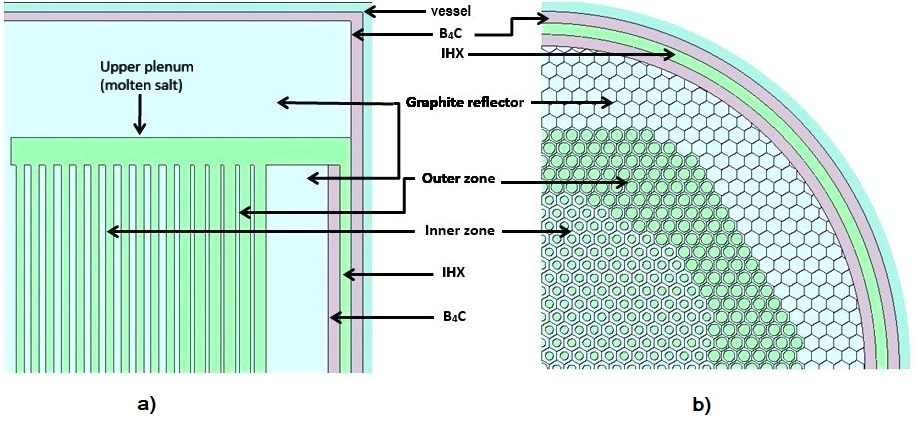
\includegraphics[width=\textwidth]{ff.png}
	\caption{$XZ$ (a) and $XY$ (b) section of the quarter-core model of the 
	SD-TMSR \cite{ashraf2019Preliminary}.}
	\label{fig:ff}
\end{figure}

\begin{table}  %[!ht]
	\caption{The main characteristics of the SD-TMSR \cite{li_optimization_2018,ashraf2019whole_core}.}
	\vspace{0.1in}
	\begin{tabularx}{\textwidth}{l | r}
		\hline
		Thermal power, MW$_{th}$          				&  2,250  \\ 
		Fuel salt components                            & LiF-BeF$_2$-(\gls{HM})F$_N$ \\
		Fuel composition, mole\%                        & 70-17.5-12.5    \\
		$^7$Li enrichment, \%        				& 99.995   \\
		Fuel temperature, K 							& 900  \\
		Fuel density at 900 K, g/cm$^3$		  		& 3.3 \\
		Fuel dilatation coefficient, g/(cm$^3$$.$K)  &  -6.7$\times$10$^{-4}$ \\
		Graphite density, g/cm$^3$             	    & 2.3	\\  
		B$_4$C density, g/cm$^3$					& 2.52  \\
		$^{10}$B enrichment, \%						&  18.4  \\
		Core diameter, cm								& 460  \\
		Core height, cm									& 460  \\
		Side length of the graphite hexagonal prism, cm   & 7.5 \\
		Inner radius, cm							& 3.5  \\
		Outer radius, cm							& 5  \\
		Ratio of molten salt and graphite in the inner zone	&  0.357  \\
		Ratio of molten salt and graphite in the outer zone &  1.162  \\
		Fuel volume, m$^3$  &	52.9 \\
		\hline
	\end{tabularx}
	\label{tab:table1}
\end{table}

\subsection{Fuel composition}
The general composition of the startup liquid fuel salt in this work is 70LiF - 
17.5BeF$_2$ - 12.5(HM)F$_N$ mole\%, where HM is the heavy metal (mixture of 
thorium and one of these fissile materials: \gls{HALEU}, Pu mixed with \gls{HALEU}, reactor-grade Pu, \gls{TRU}, and $^{233}$U), and $N$ is dependent on the chosen fissile material and the thermochemical state of the liquid fuel salt.

The aim of this paper is to simulate the  
operation of the SD-TMSR for 60 years with various startup fissile 
compositions and without any external feed of fissile $^{233}$U which we 
assume is unavailable. For that reason, five different types of initial 
fissile materials are considered based on \gls{HALEU}, Pu, and \gls{TRU} from Light Water
Reactor (LWR) spent nuclear fuel (SNF):
\begin{enumerate}[label=(\alph*)]
	\item High Assay Low Enriched Uranium (HALEU) (19.79\%),
	\item Pu mixed with \gls{HALEU} (19.79\%),
	\item reactor-grade Pu \cite{marka1993explosive},
	\item transuranic (TRU) elements from LWR SNF \cite{de2000scenarios}, and
	\item $^{233}$U for comparison \cite{ashraf2019whole_core}.
\end{enumerate}
All types of initial fissile materials are fed as fluorides.
The reactor-grade Pu and \gls{TRU} compositions are summarized in 
Table~\ref{tab:table2} and ~\ref{tab:table3}, respectively.

\begin{table} % [!ht]
	\centering
	\caption{Reactor-grade Pu vector (wt.\%) \cite{marka1993explosive}.}
	\vspace{0.1in}
	\begin{tabularx}{\textwidth}{X X X X X}
		\hline
		$^{238}$Pu & $^{239}$Pu & $^{240}$Pu & $^{241}$Pu & $^{242}$Pu \\
		\hline
		$ $ $ $ $ $ $ $ $ $1.3 &$ $ $ $ $ $60.3&$ $ $ $ $ $24.3&$ $ $ $ $ $ $ $ $ $9.1&$ $ $ $ $ $ $ $ $ $ $ $ $ $5 \\
		\hline
	\end{tabularx}
	\label{tab:table2}
\end{table}

\begin{table} %  [!ht]
	\centering
	\caption{\gls{TRU} vector (wt.\%) \cite{de2000scenarios}.}
	\vspace{0.1in}
	\begin{tabularx}{\textwidth}{X X X X X X X X X X}
		\hline
		$^{237}$Np&$^{238}$Pu & $^{239}$Pu & $^{240}$Pu & $^{241}$Pu & $^{242}$Pu&$^{241}$Am &$^{243}$Am&$^{244}$Cm &$^{245}$Cm\\
		\hline
		$ $ $ $ $ $ $ $ $ $6.3&$ $ $ $ $ $ $ $ $ $2.7& $ $ $ $ $ $45.9& $ $ $ $ $ $21.5& $ $ $ $ $ $10.7&$ $ $ $ $ $ $ $ $ $6.7&$ $ $ $ $ $ $ $ $ $3.4&$ $ $ $ $ $ $ $ $ $1.9&$ $ $ $ $ $ $ $ $ $$ $0.8&$ $ $ $ $ $ $ $ $ $0.1 \\
		\hline
	\end{tabularx}
	\label{tab:table3}
\end{table}

For the reactor-grade Pu case, the composition is taken for Pu 
recovered from the SNF composition of a commercial \gls{PWR} with an 
average discharge burnup of $33$ $GWd/tHM$ and after $10$ years of cooling before 
reprocessing \cite{oecd1989probabilistic,marka1993explosive}. Similarly, the 
isotopic compositions of \gls{TRU} reflect the composition of the \gls{PWR} UOX SNF 
(after one use, no multi-recycling) with an average discharge of $60$ 
$GWd/tHM$ burnup and after $5$ years of cooling \cite{de2000scenarios}. 
The molar composition of startup fuel for all five cases is listed in 
Table~\ref{tab:table4}. Additionally, the corresponding initial nuclei 
inventories with various fissile fuel options are summarized in 
Table~\ref{tab:table5}.
\begin{table}  %[!ht]
	\caption{Molar composition for startup fuel salts (mole\%).}
	\vspace{0.1in}
	\begin{tabularx}{\textwidth}{p{0.13\textwidth} X p{0.18\textwidth} 
	p{0.14\textwidth} X X}
		\hline
		Fuel salt component& \gls{HALEU} (19.79 wt.\%) & Pu+\gls{HALEU} (19.79 wt.\%) 
		&  reactor-grade Pu & \gls{TRU}& $^{233}$U \\
		\hline
		LiF&70.0&70.0&70.0&70.0&70.0\\
		BeF$_2$&17.5&17.5&17.5&17.5&17.5\\
		ThF$_4$&8.25&7.50&10.75&	8.65&12.3		\\
		UF$_4$&4.25&4.75&&&	0.20		\\
		PuF$_3$&&0.25&1.75&&		\\
		(TRU)F$_3$&&&	&3.85	&\\
		\hline
		Total HM &12.5&12.5&12.5&12.5&12.5\\
		\hline
	\end{tabularx}
	\label{tab:table4}
\end{table}

\begin{table}  %[!ht]
	\caption{Initial heavy metal inventories for 
	various initial fissile loadings (kg).}
	\vspace{0.1in}
	\begin{tabularx}{\textwidth}{X X p{0.18\textwidth} 
	p{0.14\textwidth} X X}
		\hline
		Nuclide & \gls{HALEU} (19.79 wt.\%) & Pu+\gls{HALEU} (19.79 wt.\%) &  
		reactor-grade Pu & \gls{TRU}& $^{233}$U \\	\hline
		$^{232}$Th       &6.24E+04 & 4.67E+04 &   6.75E+04			& 5.44E+04	& 7.69E+04    \\ 
		$^{233}$U        &         & &        &       &  1.30E+03 \\
		$^{235}$U        & 3.17E+03 &6.01E+03	&            &   & \\
		$^{238}$U      	 &1.28E+04  &2.43E+04 &	&  &\\
		$^{237}$Np	  	 &         && &1.58E+03	&    \\
		$^{238}$Pu	  	 &         &1.60E+01	& 1.13E+02 & 6.78E+02	&   \\
		$^{239}$Pu       &         &9.59E+02&6.76E+03& 1.15E+04&    \\
		$^{240}$Pu       &         &3.99E+02& 2.82E+03&5.40E+03&  	\\  
		$^{241}$Pu		 &         &1.60E+02&1.13E+03&2.69E+03&   \\
		$^{242}$Pu		 &         &6.39E+01	&4.51E+02	& 1.68E+03& \\
		$^{241}$Am		 &         &&& 8.53E+02 & \\
		$^{243}$Am       &        & &&4.77E+02&\\
		$^{244}$Cm		 &        & &&2.01E+02&  \\
		$^{245}$Cm		 &        & &&			2.51E+01	&   \\ 
		\hline
	\end{tabularx}
\label{tab:table5}
\end{table}


\section{Methodology and tools} \label{Methodology-and-tools}

Simulation of liquid-fueled Molten Salt Reactor (MSR) systems requires 
computational software that can support online fuel salt reprocessing and 
refueling \cite{serp2014molten}. In this work, SERPENT-2 version 2.1.31 \cite{leppanen2014serpent} simulates the 
SD-TMSR full-core with various initial fuel types. This extension 
of SERPENT accounts for continuous online reprocessing and refueling 
\cite{aufiero2013extended}. The ENDF-VII.0 cross section library was used for all 
calculations in this work. The results demonstrate full-core runs of
$1.25\times 10^7$ neutron histories per depletion step. During the depletion step, the core was maintained critical and total fuel mass was almost constant (dm $\leq$ 0.1\%). To determine the appropriate depletion step size, we conducted a time step refinement study. We started with $\Delta t=30$ days and gradually increased the depletion time step until the error in K$_{eff}$ became significant. The difference in $k_{eff}$ between $\Delta t=1$ year and $\Delta t=30$ days was $\leq$ 0.02\%; thus, we adopted a constant, 365-day-long time step for all simulation in this work.
The full burnup time of 
the SD-TMSR was 60 years with statistical error in $k_{eff}$ equal to $\pm$ 
$12$ $pcm$. 
During the molten salt reactor operation, part of fuel salt flows outside of the reactor core then the fission reaction has not happened in the external loop, however, the decay reactions happen everywhere. We used total fuel salt inventory in the primary loop to define the fuel material in the SERPENT input. Moreover, we accordingly adjusted power density in SERPENT burnup calculations because fission takes place only in the core region. But we did not consider processes, such as decay, which occurs outside of the core. Also, the drift of the delayed neutron precursors is not examined in this paper, but discussion about this can be found in \cite{zhang2018review}.     

The liquid fuel is well-mixed all the time due to turbulent flow and mixing in the pump. We used the depletion mode 1 in SERPENT-2 (i.e. burn 1), which means that the fuel material is treated as a single depletion zone. 

The online extraction of \gls{FPs} and other neutron absorbers 
provides many benefits for MSRs. For example, it has the potential to reduce the initial 
fissile material inventory required to achieve criticality and improve the 
breeding ratio. Figure~\ref{fig:flow} shows a flow chart of the calculation 
steps. 

\begin{figure}[t!] % replace 't' with 'b' to \centering
	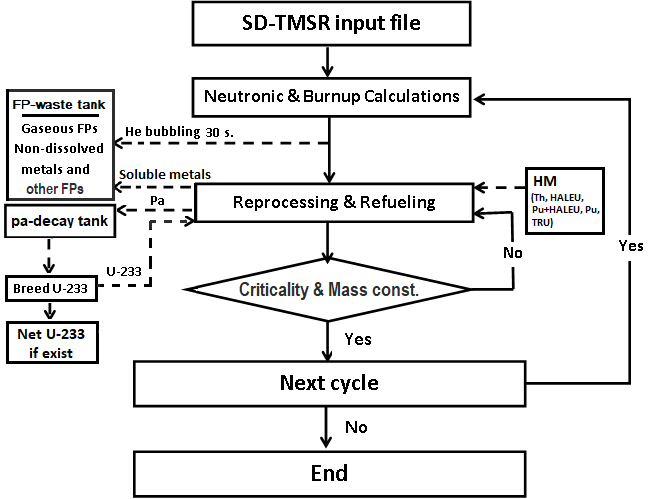
\includegraphics[width=\textwidth]{flowch1.png}
	\caption{Flow chart of the calculation procedures (implemented by SERPENT-2).}
	\label{fig:flow}
\end{figure}

As shown in Figure~\ref{fig:flow}, after launching the input file, SERPENT solves the Bateman equation using an advanced 
matrix exponential solution based on the Chebyshev Rational Approximation 
Method \cite{isotalo2016improving}. 
Then, the system extracts gaseous \gls{FPs} and other materials 
(non-dissolved metals, lanthanides, and soluble metals except Pa) with 
a suitable removal rate\footnote{The extraction rate depends on the type of 
poison and its impact on the neutron
economy.}. This is done by setting the 
flow rate of gaseous \gls{FPs} and other materials from the fuel to the 
\texttt{FP-waste tank}\footnote{An external tank used to store the gaseous 
\gls{FPs} and the other materials (non-dissolved metals, lanthanides, and 
soluble metals except protactinium).}. Specifically, Pa is removed 
from the fuel with a certain flow rate into the 
\texttt{Pa-decay tank} to decay and produce $^{233}$U \footnote{The 
$^{233}$Pa is removed and left to decay into $^{233}$U with $\tau_{1/2}$ 
$\approx$ $27$ $d$.}. The produced $^{233}$U is used as a fresh fissile fuel 
and the residual $^{233}$U (if exist) is the net production of $^{233}$U that required to start up a new SD-TMSR and achieve the transition to thorium fuel cycle. The MSR burnup 
routine provided by SERPENT-2 allows changes to the mass flow rates ($mflow$) of the 
isotopes during reactor operation \cite{aufiero2013extended}. Specifically, the SERPENT user should determine the mass flow rate ($mflow$), which is the rate by 
which elements or nuclides are transferred between materials. After that, the 
flow rates must be connected to materials with a reprocessing scheme. 
The final step is to link the reprocessing schemes to depletion histories. In 
the present work, we adjust the transfer rates of fresh fuel to maintain core 
criticality and to keep fuel salt mass constant during burnup. The continuous feed constant calculation procedures are summarized as follows:
\begin{enumerate}
	\item The simulation starts without injecting refueling materials (i.e. only removing FPs and Pa).
	\item After the first depletion calculation step, we check the total mass density of FPs and Pa in the \texttt{FP-waste tank} and \texttt{Pa-decay tank}, respectively.
	\item A simple calculation yields the amount of heavy metal that must be added during this cycle:
	\subitem 3a. \textbf{Thorium feed mechanism}: mass of injected $^{233}$U 
	$\approx$ mass of extracted Pa and mass of injected $^{232}$Th $\approx$ 
	mass of extracted FPs to maintain the total fuel mass constant.
	\subitem 3b. \textbf{Non-thorium feed mechanism}: mass of injected $^{233}$U $\approx$ mass of extracted Pa and mass of injected fuel (i.e., HALEU, Pu mixed with HALEU, reactor-grade Pu, or TRU) $\approx$ mass of extracted FPs to maintain the total fuel mass constant.
	\item Dividing this mass by time and inventory of refueling material gives the corresponding feed constant (1/s).
\end{enumerate}
In both feed mechanisms (thorium and non-thorium) we continuously added 
$^{233}$U and the mass of injected $^{233}$U is equal to the mass of extracted 
Pa ($^{233}$Pa decays to $^{233}$U after $\approx$ 27 d). To keep the total 
fuel mass almost constant, for \textbf{thorium feed mechanism}, the mass of 
injected thorium must be equal to the mass of extracted FPs and for 
\textbf{non-thorium feed mechanism}, the mass of injected fuel (i.e., HALEU, 
Pu mixed with HALEU, reactor-grade Pu, or TRU) must be equal to the mass of 
extracted FPs.

\section{Feed and extraction rates} \label{Feed-and-extraction-rates}
In the present work, two different feed mechanisms are used: (1) thorium and (2) non-thorium.
The first mechanism allows continuous feed flow of thorium from the external stockpile and 
$^{233}$U from the \texttt{Pa-decay tank}. In contrast, the second mechanism 
continuously injects external heavy metals (\gls{HALEU}, Pu mixed with \gls{HALEU}, reactor-grade Pu, \gls{TRU}) and simultaneously feeds  
all or part of produced $^{233}$U from the \texttt{Pa-decay tank}. The fission 
products (FPs) act as poisons in nuclear reactors: they negatively impact the reactivity. 
Therefore, \gls{FPs} must be extracted during reactor operation. Consider 
the \gls{MSR} extracts $dN_{e}$ amount of particular element $e$ during time $dt$, thus \cite{nuttin2005potential}:
\begin{align}
\dfrac{dN_{e}}{dt} &= N_{e}\dfrac{\varepsilon_{e}}{T_{r}}
\label{Equ:1}
\intertext{where}
dN_{e} 	&= \mbox{the amount of particular element $e$} \nonumber \\
dt   	&= \mbox{the extraction time of $dN_e$} \nonumber \\
N_{e}  	&= \mbox{total inventory of element $e$} \nonumber \\
\varepsilon_{e}	&= \mbox{the removal efficiency $\%$} \nonumber \\
T_{r}	&= \mbox{the time during which the total fuel salt is reprocessed.} \nonumber
\end{align}

Integration of equation \ref{Equ:1} gives the removal constant $\lambda_{e}$ $[s^{-1}]$ (the rate at which the material 
is removed), where $\lambda_{e}=\dfrac{{\varepsilon_{e}}}{{T}_{r}}$. The removal constant 
$\lambda_{e}$ of gaseous and other fission products is precisely calculated 
and summarized in Table~\ref{tab:table6}. The effective reprocessing time for 
the gaseous \gls{FPs} and non-dissolved metals was set to 30 s (removal 
constant $\lambda_{e}$ = $-0.0333$ $s^{-1}$), because such elements must be 
extracted promptly and continuously via a gas removal system. In contrast, 
chemical processes (i.e. fluorination and reduction) extract the soluble \gls{FPs}, lanthanides, and Pa.
Therefore, the system reprocesses a specific amount of fuel salt daily. In the 
present work, the effective extraction time for soluble \gls{FPs} is 
$\approx$10.59 days ($\lambda_{e}$ = $-1.092\times10^{-6}$ $s^{-1}$), which is 
equivalent to a chemical reprocessing rate of 5 m$^3$/d chosen by Nuttin \emph{et al.} \cite{nuttin2005potential} and Li \emph{et al.} \cite{li_optimization_2018}. The effective feed rates of 
the heavy metals (HM) are changed during reactor operation to conserve the 
total fuel mass and criticality. The effective feed rates for Th/$^{233}$U, reactor-grade Pu, and TRU cases are listed in Table A.1, A.2, and A.3 in \ref{Appendix}.


\begin{table}[ht!]
	\centering
	\caption{The reprocessing table \cite{ashraf2019whole_core,ashraf2019Preliminary}.} 
	\vspace{1ex}
	\begin{tabularx}{\textwidth}{|p{2.3cm}|p{4cm}|p{2.2cm}|p{1.9cm}|}
			\hline
			\textbf{Reprocessing group}  & \textbf{Element} & \textbf{Reprocessing time} & \textbf{Removal constant} $\lambda_{e}$ $[s^{-1}]$ \\
			\hline
			\raggedright Gaseous \gls{FPs} and non-dissolved metals  &  H, He, N, O, Ne, Ar, Kr, Nb, Mo, Tc, Ru, Rh, Pd, Ag, Sb, Te, Xe, Lu, Hf, Ta, W, Re, Os, Ir, Pt, Au, and Rn.		&	\raggedright 30 s	&  -3.333E-02 \\
			\hline
			\raggedright Lanthanides and other soluble \gls{FPs}     & 
			Zn, Ga, Ge, As, Se, Br, Rb, Sr, Y, Zr, Cd, In, Sn, I, Cs, Ba, La, Ce, Pr, Nd, Pm, Sm, Eu, Gd, Tb, Dy, Ho, Er, Tm, and Yb. & \raggedright 10.59 d (5 m$^3$/d) &  -1.092E-06 \\
			\hline
			Protactinium   & Pa  & \raggedright 10.59 d (5 m$^3$/d)  &  -1.092E-06 \\
			\hline
	\end{tabularx}
	\label{tab:table6}
\end{table}